\documentclass{beamer}
\usepackage[ngerman]{babel}
\usepackage[ansinew]{inputenc}
\usepackage{csquotes}
\usepackage{url}
\usepackage{graphicx}
\usepackage{amsmath}
\usepackage{amssymb}
\usepackage{nicefrac}
\usepackage{eurosym}
\usepackage{xcolor}
\usepackage{alltt}
\usepackage{tikz}
\usepackage{ragged2e} 
\usepackage{tabu}
\usetikzlibrary{trees}
\usepackage{calc,color,colortbl,nicefrac}
\newtheorem*{bem}{Bemerkung}
\usepackage{multirow}

%smaller footnotes
\renewcommand{\footnotesize}{\tiny}
%reduce spacing in footnotes
\setlength{\footnotesep}{0em}

%use for inline citation formatting
\newcommand{\textct}[1]{{\textsuperscript{\tiny \color{gray}#1}}}

\newlength{\myX}
\newlength{\myY}

%absolute figure positioning
\usepackage[absolute,overlay]{textpos}
  \setlength{\TPHorizModule}{1mm}
  \setlength{\TPVertModule}{1mm}

%quote environment with reference 
\def\signed #1{{\leavevmode\unskip\nobreak\hfil\penalty50\hskip2em
  \hbox{}\nobreak\hfil(#1)%
  \parfillskip=0pt \finalhyphendemerits=0 \endgraf}}
\newsavebox\mybox
\newenvironment{aquote}[1]
  {\savebox\mybox{#1}\begin{quote}}
  {\signed{\usebox\mybox}\end{quote}}

\definecolor{purp}{HTML}{3333b3}
\definecolor{dgrey}{rgb}{0.8,0.8,0.8}
\definecolor{bgrey}{rgb}{0.95,0.95,0.95}

\usepackage{graphicx}
\graphicspath{{img/}}

\newlength{\stdlength}
% Standardlaenge fuer Skript und Folien
\setlength{\stdlength}{8cm}

\usetheme{Copenhagen}
\usefonttheme{professionalfonts}
\usecolortheme{default}

\bibliography{literature}
\usepackage[style=authoryear, backend=bibtex]{biblatex} 
\addbibresource{literature.bib}

\defbibenvironment{bibliography}
{\list{}
{\setlength{\leftmargin}{\bibhang}%
\setlength{\itemindent}{-\leftmargin}%
\setlength{\itemsep}{6px}%
\setlength{\parsep}{\bibparsep}}}
{\endlist}
{\item \scriptsize}

\definecolor{mygrey}{RGB}{80,80,80}

\setbeamertemplate{headline}
{%
\hfill
\textbf{\insertsection} \
\insertsubsection \
\insertframenumber / \inserttotalframenumber
}
\setbeamertemplate{navigation symbols}{}

\title{Bewegungsvorhersage mittels mobiler Endger�te}
\author{
Sebastian B�r, Frank Rosner
}

\institute{
Martin-Luther-Universit�t Halle-Wittenberg
}
\date{10. Juli 2013}

\begin{document}

\frame{\titlepage 
\parbox{0cm}{\tiny 
\vspace{-30pt}\color{mygrey}
\begin{tabbing}
XXXXXXXXXXXXXXXXXXXXXX\=XXXXXXXXXXX\= \kill \\
\>Veranstaltung:\> "`Seminar zum E-Business"'\\
\\
\>Dozenten:\> Prof. Dr. Ralf Peters\\
\>\> Dr. Thomas W�hner\\
\>\> Sebastian K�hler\\
\>\> Uwe Bretschneider\\

\end{tabbing}
}
}

\begin{frame}
\frametitle{Gliederung}
\tableofcontents
\end{frame}

\section{Einleitung}
\frame{\frametitle{Gliederung} \tableofcontents[currentsection]}

\begin{frame}{Problemstellung}
\begin{itemize}
\item Computer allgegenw�rtig
	\begin{itemize}
	\item[$\Rightarrow$] mobile Endger�te
	\item[$\Rightarrow$] "`ubiquitous computing"'
	\end{itemize}
\item Positionsbestimmung relativ genau m�glich
\end{itemize}

\begin{itemize}
\item wirtschaftlicher Nutzen?
	\begin{itemize}
	\item[$\Rightarrow$] positionsabh�ngige, personalisierte Dienste
	\item[$\Rightarrow$] z.B. Mittagskarte eines Restaurants in der N�he
	\end{itemize}
\end{itemize}

\begin{itemize}
\item Positionsvorhersage statt Positionsbestimmung?
	\begin{itemize}
	\item[$\Rightarrow$] positionsabh�ngige Dienste im Voraus bereitstellen
	\item[$\Rightarrow$] Mittagskarte des Restaurants, wenn ich mich gerade auf dem Weg dorthin befinde
	\end{itemize}
\end{itemize}

\begin{textblock}{70}(100,25)
	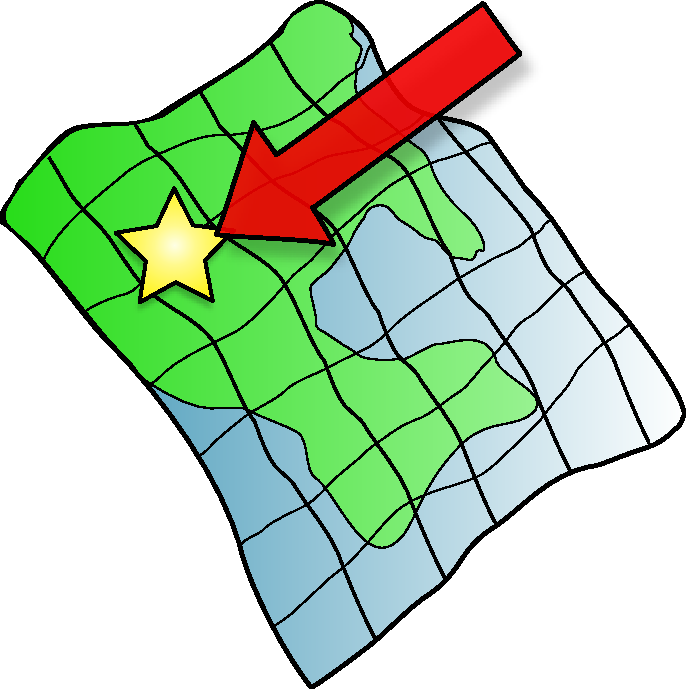
\includegraphics[width=2cm]{ruffled_map.pdf}
\end{textblock}

\end{frame}

\begin{frame}{Zielstellung und Methodik}
\textbf{Zielstellung}
\begin{itemize}
\item Android-App zur Bewegungssdatensammlung entwickeln
\item Auswerten der Positions- und Bewegungsdaten
	\begin{itemize}
	\item[$\Rightarrow$] Visualisierung
	\item[$\Rightarrow$] Vorhersage
	\end{itemize}
\end{itemize}

\vspace*{1em}

\textbf{Methodik}
\begin{itemize}
\item Softwareentwicklung
\item Datensammlung
\item Statistische Auswertung
\end{itemize}
\end{frame}

\section{Datensammlung}
\frame{\frametitle{Gliederung} \tableofcontents[currentsection]}
\begin{frame}{Android �berblick}
\begin{figure}[h]
\centering
%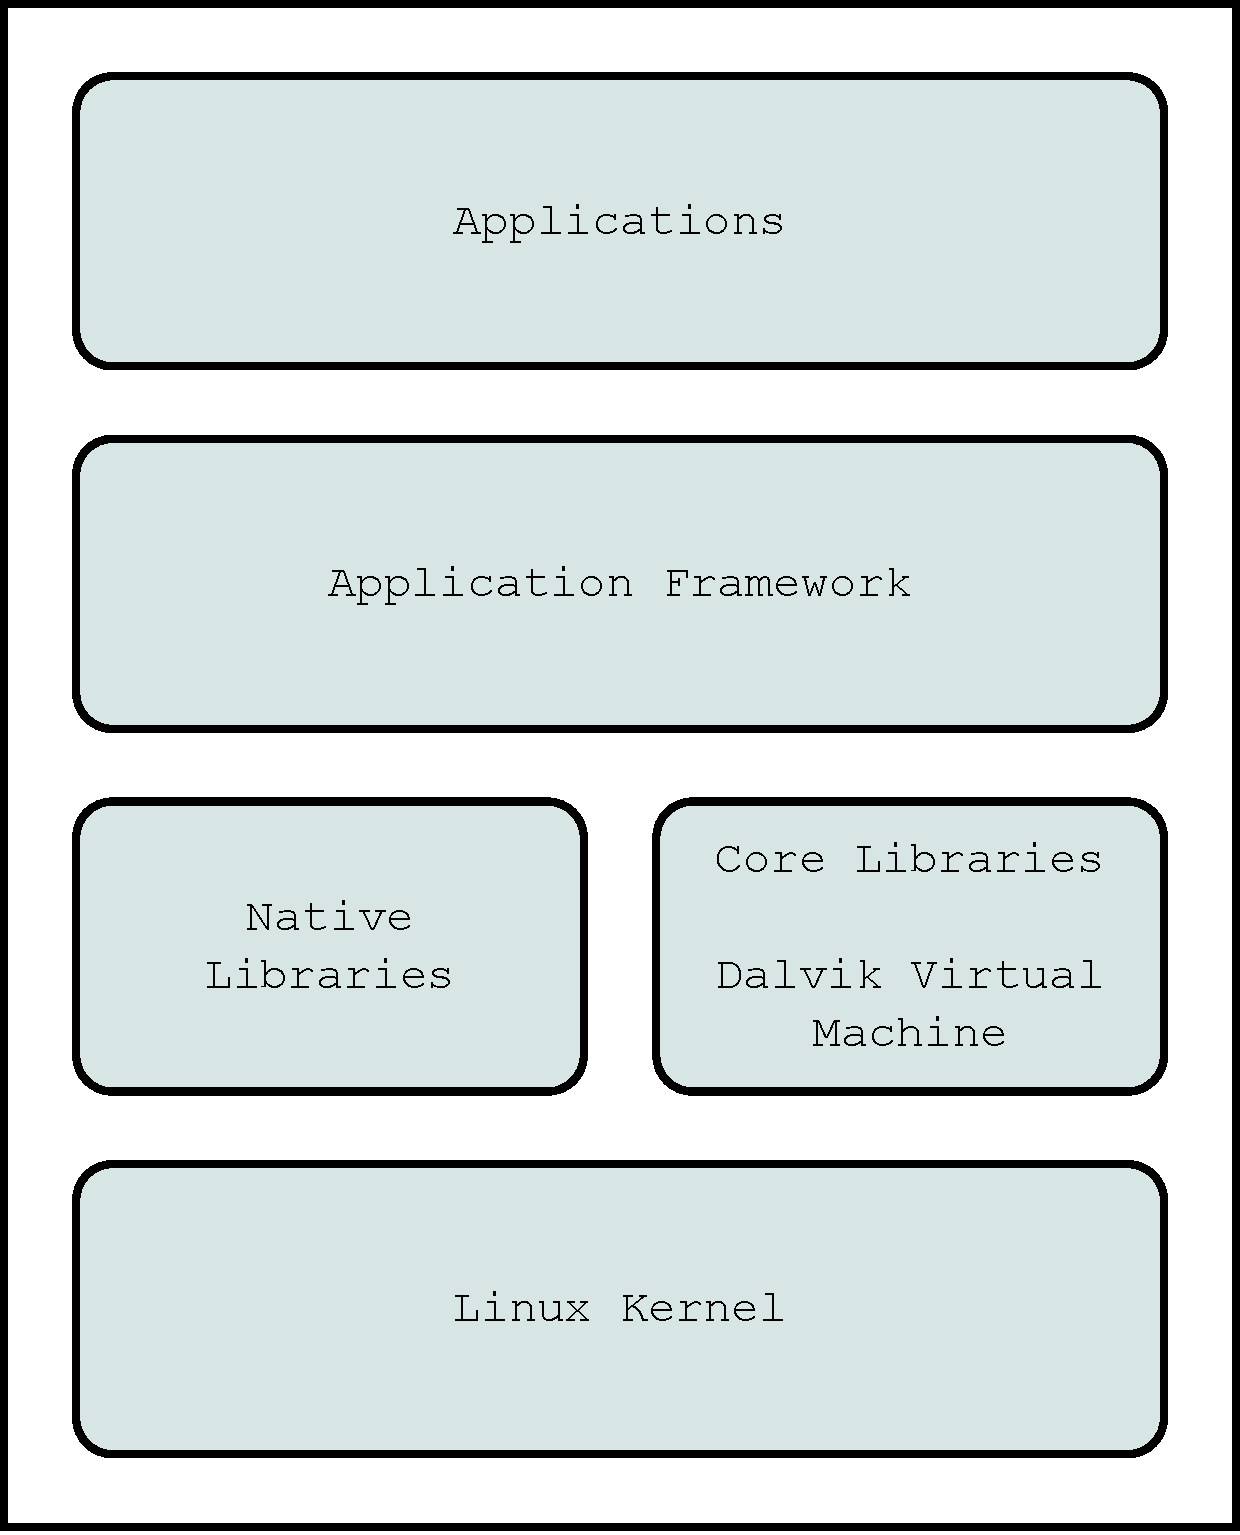
\includegraphics[height=60mm]{img/android_stack.pdf}
\caption[Android Stack]{Android Stack, Quelle: }
\end{figure}
\end{frame}

\begin{frame}{Android-SDK}
\begin{itemize}
\item enth�lt Eclipse als IDE
\item Debug-Treiber zur Anbindung von Ger�ten
\item Emulator zum Testen
\item Debug-Monitor
\item Layout-Editor
\item SQLite Datenbank-Treiber
\item XML-Editor
\end{itemize}
\end{frame}

\begin{frame}{Aufbau einer Applikation}
\begin{itemize}
\item die Activity �bernimmt Darstellung des User-Interface sowie Ausf�hrung von Logik
\item ein Service �bernimmt Aufgaben im Hintergrund
\item Intents sind abstrakte Beschreibungen von Operationen, die eine App ben�tigt und eine andere anbieten kann
\item BroadcastReceiver warten auf Intents und verarbeitet diese
\item AndroidManifest enth�lt Informationen dar�ber welche Android-Versionen unters�tzt werden, Versionen der App, welche Berechtigungen n�tig sind
\item dar�ber hinaus wird ein Layout-XML ben�tigt
\end{itemize}
\end{frame}

\begin{frame}{Aufbau AndroidDataCollection}
\begin{figure}[h]
\centering
%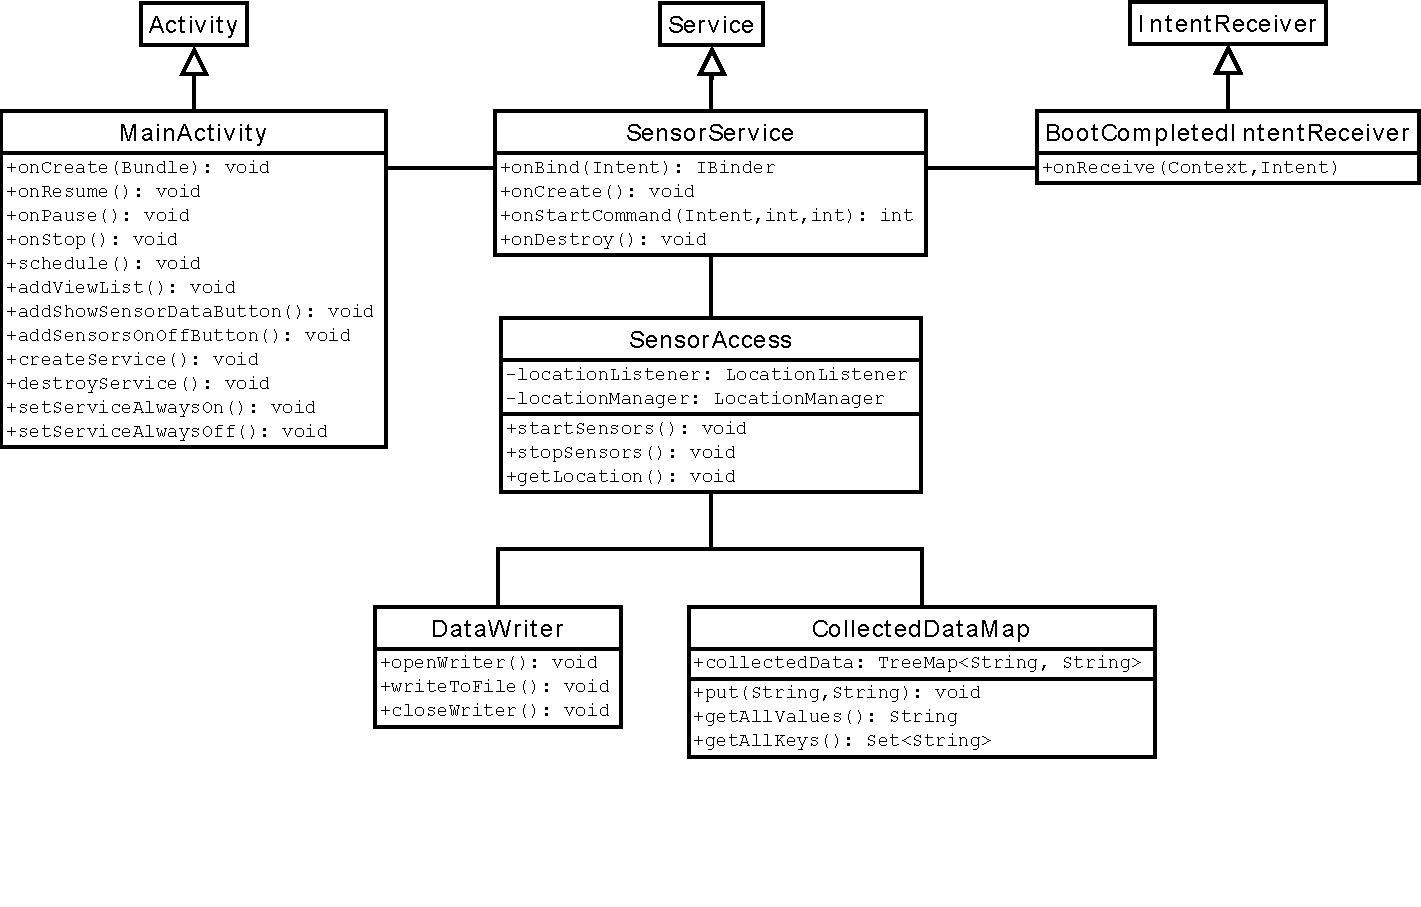
\includegraphics[height=60mm]{img/class_diagram.pdf}
\caption[Android Stack]{Klassendiagramm, Quelle: }
% Lebenszyklus einzelner Komponenten ansprechen
\end{figure}
\end{frame}

\begin{frame}{Benutzeroberfl�che}
\begin{figure}[h]
\centering
%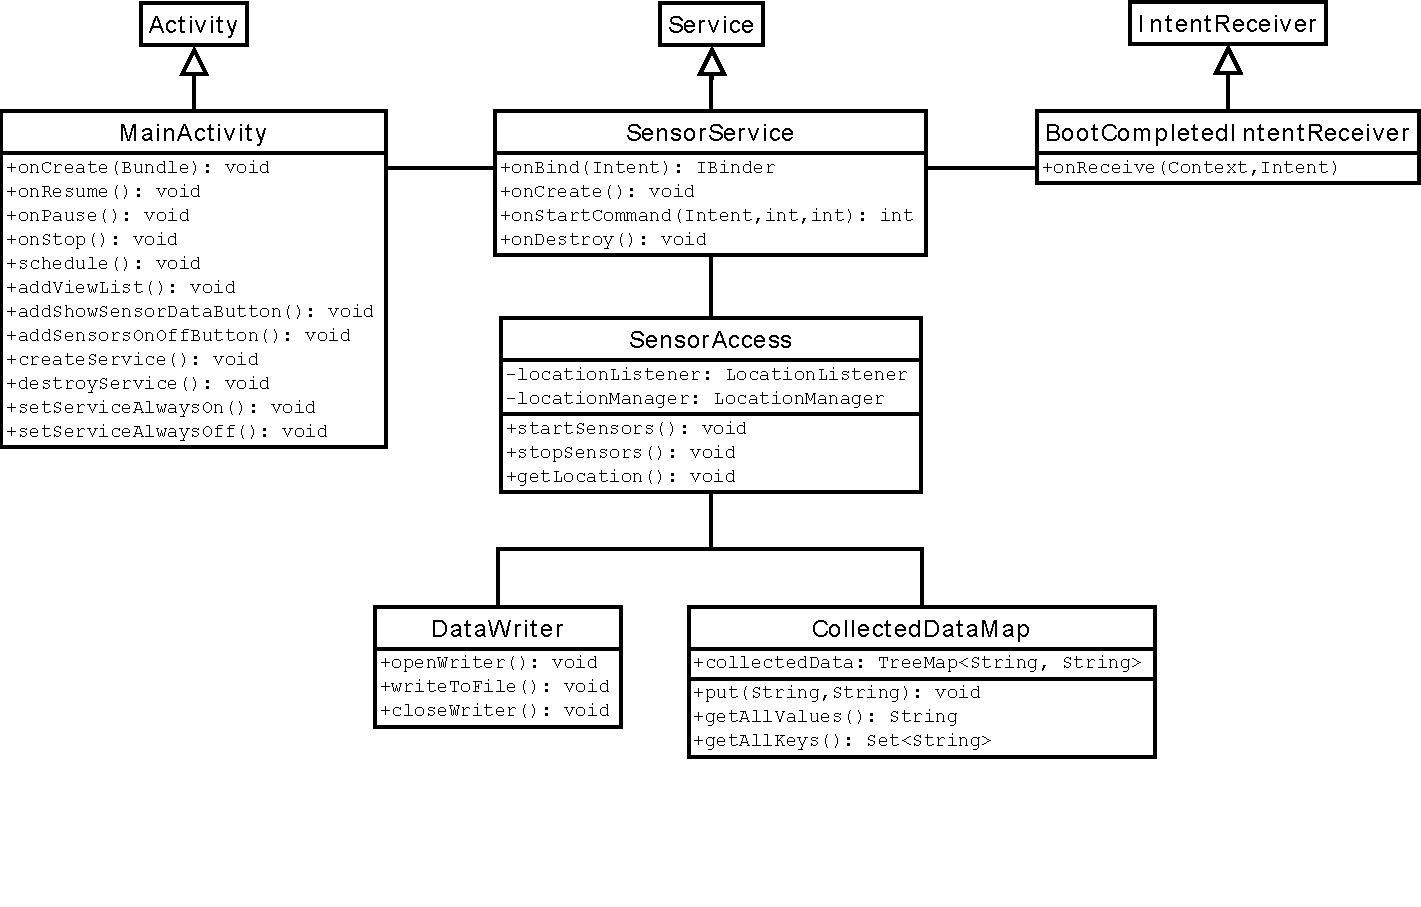
\includegraphics[height=60mm]{img/class_diagram.pdf}
\caption[Benutzeroberfl�che]{Benutzeroberfl�che, Quelle: }
% Lebenszyklus einzelner Komponenten ansprechen
\end{figure}
\end{frame}

\begin{frame}{AndroidManifest}
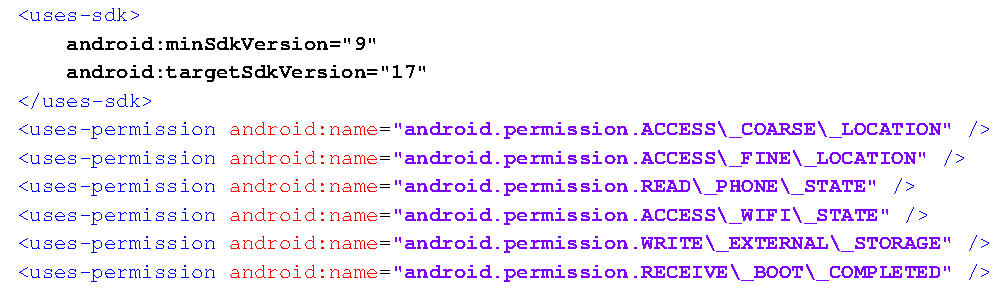
\includegraphics[width=1\linewidth]{android_manifest_cropped.pdf}
\end{frame}

\begin{frame}{MainActivity}
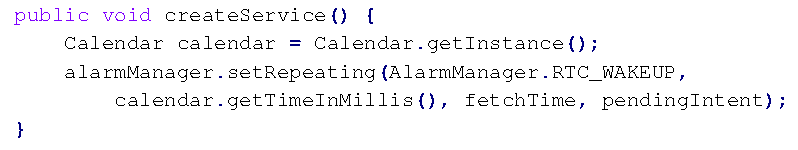
\includegraphics[width=1\linewidth]{createService_cropped.pdf}
\end{frame}

\begin{frame}{SensorService}
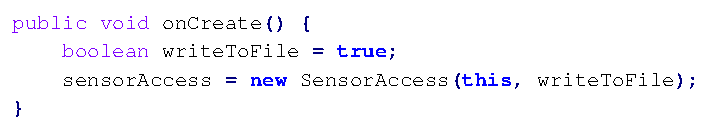
\includegraphics[width=1\linewidth]{onCreate_cropped.pdf}

\end{frame}

\begin{frame}{SensorService}
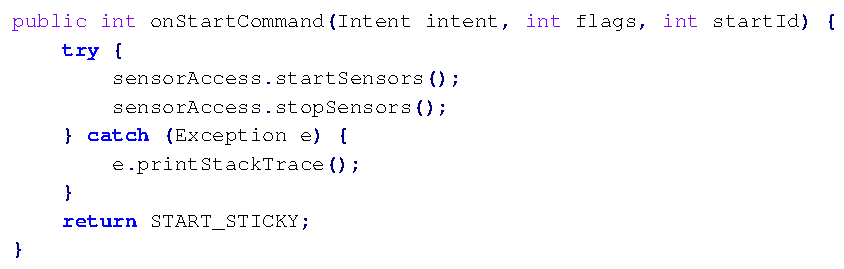
\includegraphics[width=1\linewidth]{onStartCommand_cropped.pdf}
\end{frame}

\begin{frame}{SensorAccess}
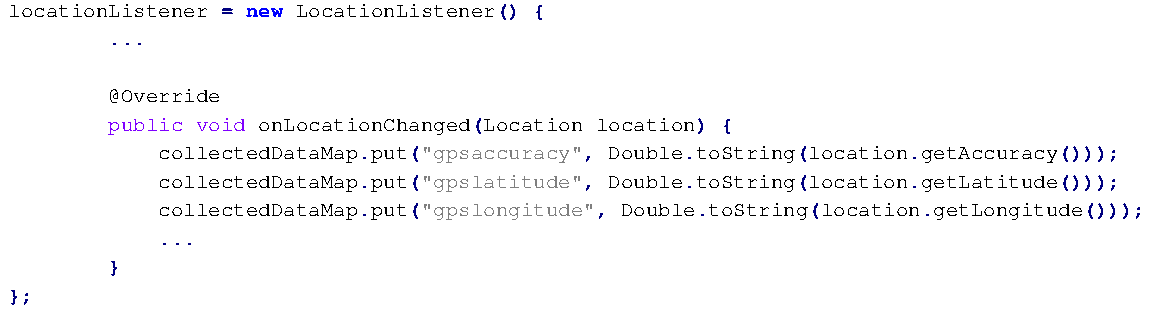
\includegraphics[width=1\linewidth]{getLocation_cropped.pdf}
\end{frame}

\begin{frame}{BootCompletedIntentReceiver}
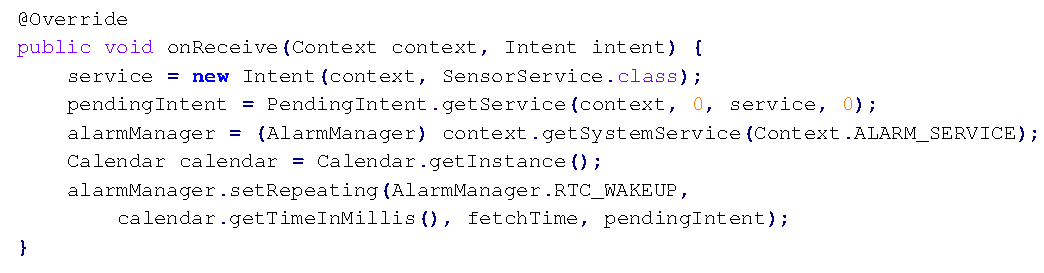
\includegraphics[width=1\linewidth]{onReceive_cropped.pdf}
\end{frame}


\section{Bewegungsvorhersage}
\frame{\frametitle{Gliederung} \tableofcontents[currentsection]}

\section{Ergebnisse}
\frame{\frametitle{Gliederung} \tableofcontents[currentsection]}

\section{Schlussbetrachtung}
\frame{\frametitle{Gliederung} \tableofcontents[currentsection]}

\section{Quellen}
\frame{\frametitle{Gliederung} \tableofcontents[currentsection]}
\begin{frame}[allowframebreaks]
\frametitle{Quellen}
\def\bibfont{\scriptsize}
\printbibliography
\end{frame}

% cite all resources to be printed in bibliography
% this frame will not be shown
\begin{frame}<0>
\frametitle{Quellen}

\end{frame}

\begin{frame}
\thispagestyle{empty}
\begin{center}
\Huge
Vielen Dank f�r Ihre Aufmerksamkeit!\\
Fragen?
\end{center}
\end{frame}

\end{document}



